\section{Implementation}
As this was part of our access management platform we implemented this floorplan also in our web application.

\begin{figure}[!hb]
	\centering
	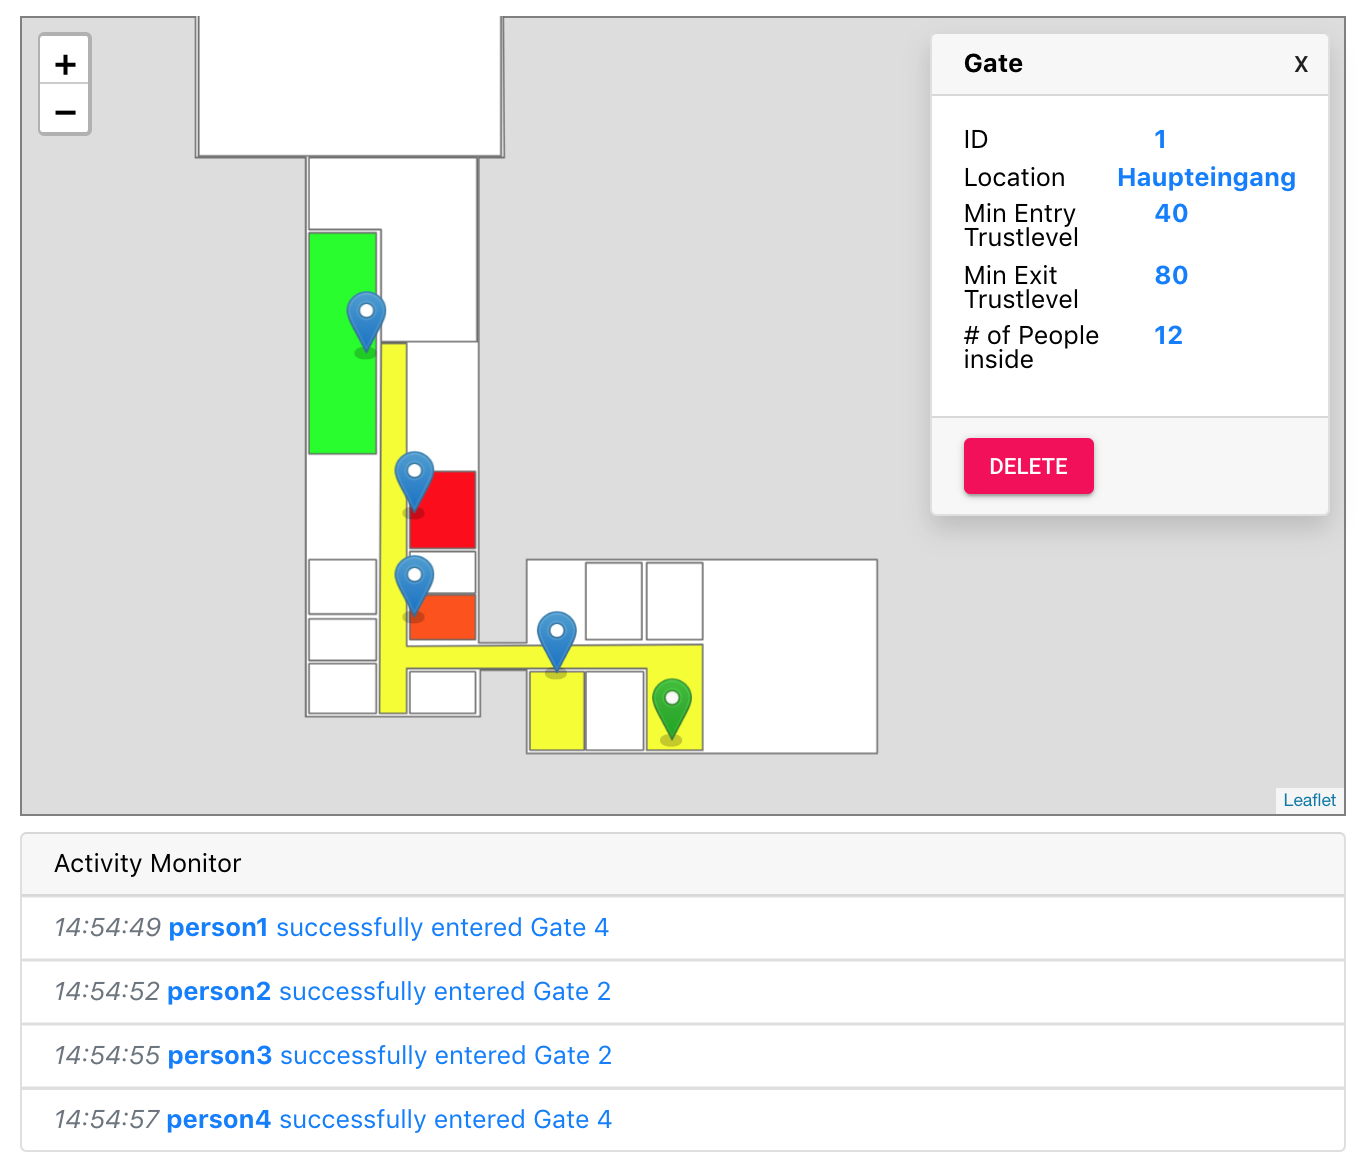
\includegraphics[width=0.9\linewidth]{images/FloorplanScreenshot}
	\caption{Implemented interactive floorplan}
	\label{fig:FloorplanScreenshot}
\end{figure}

\subsection{Technology Discussion}

\subsubsection{Google Maps}
\label{Google Maps}

In March 2011, Google introduced the first indoor floorplans in their map. The intention was to increase the overview in public areas like train stations, malls and airports.
Users can upload own floorplans (valid formats include for example PNG, PDF or JPEG) to the map, with restriction to only publicly available areas.

Google Maps also offers a very popular API for their services. This allows the integration of the Google Maps Services in your own website. The usage is free for commercial use up until 28000 calls per day\footnote{According to \url{https://cloud.google.com/maps-platform/pricing/sheet/?hl=de}} and requires an API key.
The Maps JavaScript API comes with direct support for importing GeoJSON and can be customized with own content. Its designed to load maps quickly and is optimized for mobile use. Aside from that it also offers a versatile visualization library, which also includes a Heatmap Layer that helps with visualizing a heatmap (Figure 2.1.).

\begin{figure}[!hb]
	\centering
	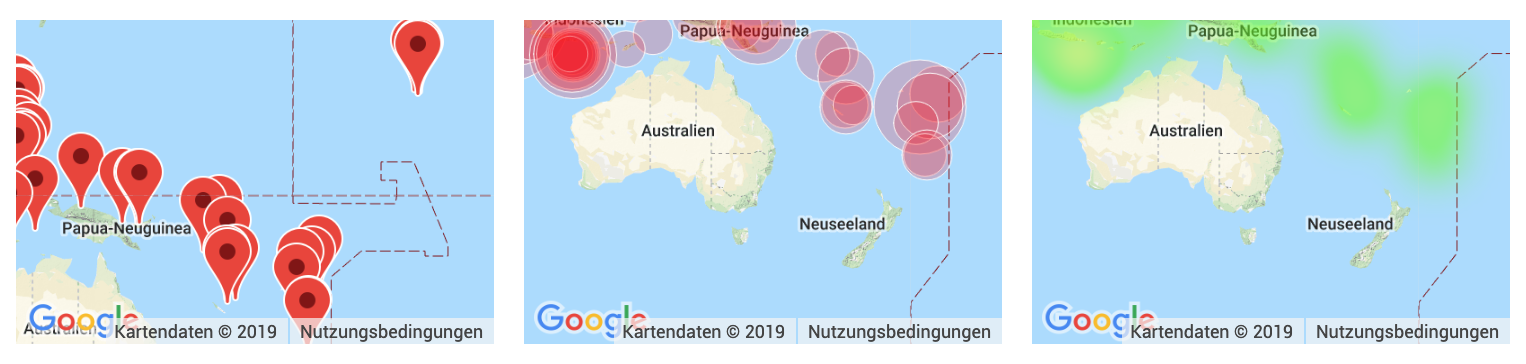
\includegraphics[width=1\linewidth]{images/GoogleMapsHeatmap}
	\caption{Example of visualization options in Google Maps}
	\label{fig:GoogleMapsHeatmap}
\end{figure}

Although this looks very promising for creating our indoor floorplan, there are quite a few problems for us.

Because the API needs an internet connection, offline development is not possible. 
Furthermore the Google Maps API would request payment after hitting the threshold of API calls mentioned above and therefore needs to be linked to an account where billing is activated. Although hitting this threshold could only happen in production, our project partner set the requirement to only use free and also open-source software and linking a billing account of our partner to use the API was not possible. 

Therefore Google Maps was not applicable to our task of creating an interactive floorplan.

\subsubsection{OpenLayers}
\label{OpenLayers}

OpenLayers is an open-source JavaScript library for displaying interactive maps. Out of the box it comes with various features like map rotation, direct mobile support and import of GeoJSON, TopoJSON, KML\footnote{Keyhole Markup Language} or GML\footnote{Geography Markup Language} data \footnote{\url{https://openlayers.org/}}. Unlike Google Maps, OpenLayers is a pure client-side library with no server-side dependencies. 

Because it has a lot of features already bundled together, it offers far more functionality than we need to meet the requirements of our floorplan. 

This also results in a heavyweight module. With a minified bundle size of 330.1 kB (Version 5.3.3) it takes up to 1.6 seconds to download on 3G\footnote{\url{https://bundlephobia.com/result?p=ol@5.3.3}}. Although this can be lowered for production by deleting unused modules, it takes extra effort to see which modules are really not used.

Due to the limited time we had for the implementation of the floorplan (due to it being the last feature on our roadmap) and only beginner knowledge of JavaScript, we needed something that is easy to understand and lets beginners output something useful in a short time. Because the abstraction layer of OpenLayers  is quite low, the learning curve can be pretty steap. Compared to Leaflet it takes a lot more code to get the same results.

Therefore we thought that OpenLayers doesn't fit our task.

\subsubsection{Leaflet}
\label{Leaflet}

Leaflet is another open-source JavaScript library for creating interactive maps. With it's first version released in 2011, it is a well established and tested library. 

By only including core features for map visualization, it only has a bundled size of 138.6KB\footnote{\url{https://bundlephobia.com/result?p=leaflet@1.5.1}}, making it a very lightweight library.

Furthermore Leaflet supports every browser and can easily be extended by plugins from the community.
This also includes plugins for creating indoor maps \cite{baines_provides_2019} and real-time maps with Socket.IO.

\subsubsection{GeoJSON}
\label{GeoJSON}

GeoJSON is a format for interchanging geospatial data and is based on JavaScript Object Notation. With the publishing of RFC 7946 in August 2016 it has a standardized format specification.
Different Geometries can be represented in a GeoJSON file. These include for example Lines, Linestrings, Polygones or Multipolygones\footnote{\url{https://tools.ietf.org/html/rfc7946}}. 

This can be used to encode the geometry for countries, houses and streets on a map, but also for encoding data for indoor rooms, stairs and hallways.


\subsection{Display of indoor features}
\label{Display of indoor features}

The indoor map plugin extends Leaflet by an |Indoor| class, which is able to load in geospatial data from a GeoJSON file:

\begin{lstlisting}[label=setupMap]
...
this.map = L.map('floorplan-container', {
            center: new L.LatLng(49.41873, 8.67689),
            zoom: 20,
        });

        const indoorLayer = new L.Indoor(this.props.geoJSON, {
        ...
\end{lstlisting}

This renders the GeoJSON data on a map with a HTML layer for each feature.

\emph{TODO: latitude, longitude erklaeren}

%Considering the limited time we had for the implementation, we decided that Leaflet fits our needs the best and could be the fastest way to build our interactive live floorplan.


Hier erwaehnen das jedes feature eine ID benoetigt und so.

\subsection{Interactive Floorplan}
\label{Interactive Floorplan}

The floorplan handles mouse clicks on each room that is displayed. If a click event occurs, it adds a new marker at this position, which is then automatically linked with the room where the click occured.

\begin{lstlisting}[label=addMarkers]
handleClickOnRoom = (event) => {
        this.addMarker(
          event.latlng, 
          { gateId: undefined, assignedRoomId: event.target.feature.id }, 
          true);
    };
\end{lstlisting}

To create this connection between the room and the marker, each feature/room in the GeoJSON file has to have a distinguashble member attribute \emph{id}. This is still following the GeoJSON format specification.

After setting the marker it needs to be linked with a gate. This is done by a selection input.

\emph{Bild rein von selection}



\subsection{Logging of Gate Events}
\label{Logging of Gate Events}

\subsubsection{Elastic Stack}
\label{Elastic Stack}

The Elastic Stack consists of mainly three open-source projects: \emph{Elasticsearch}, \emph{Logstash} and \emph{Kibana}.
Together they form a pipeline that can be used to analyze, search and visualize logs created from different sources. 

The component of the first stage of this pipeline is Logstash, which is responsible for collecting data from different locations and transforming it for the next step. Elasticsearch then indexes these logs and provides a RESTful API for searching. Kibana uses this API from Elasticsearch to provide meaningful visualization of the logs.
Through a smart indexing technology the Elastic Stack promises a fast response time even for large data sets and is used by companies like Netflix for monitoring security related logs or Medium for debugging production issues \footnote{\url{https://hackernoon.com/elastic-stack-a-brief-introduction-794bc7ff7d4f}}.

In our project logs sent from the gates need to be analyzed and visualized to give the FM Team more insights about the access decisions made. These informations get also displayed in the floorplan and the heatmap gets calculated based on the gate event logs. To ensure a fast display of the access decision data and to also ensure the possibility in the future to search and visualize logs not only from the gates, but from other sources also, we decided to include the Elastic Stack into our project.

\subsubsection{Elasticsearch Server}

Since we're working with own custom visualization, we will ignore Kibana for our implementation. And since we're only receiving events  from one source - the gates, we can skip the Logstash pipeline and send event data directly to the Elasticsearch server, which then will be stored in a database and indexed.

Since data of any form can be sent to the Elasticsearch server, it performs an automatic type detection for each property that is sent. This can result in wrong datatypes, causing the server to reject future events because they're not fulfilling the required datatypes\footnote{For example: The first event has a member id with the value "1234", then Elasticsearch will automatically cast it to an Integer. If the following event now has an id of "fe123d" Elastic will not accept the event.} To prevent this, we first have to create a template for our gate event objects, which strictly declares the datatypes for each property in the event object:

\begin{lstlisting}[label=curlScriptTemplateElastic]
curl -v -X PUT 'localhost:9200/_template/gates' -H 'Content-Type: application/json' -d '
{
  "index_patterns" : ["gates"],
  "settings": {
    "number_of_shards": 1
  },
  "mappings": {
    "_source": {
      "enabled": true
    },
    "properties": {
      "timestamp": { "type": "date" },
      "loglevel": { "type": "keyword" },
      "gateId": { "type": "keyword" },
      "deviceId": { "type": "keyword" },
      "accessType": { "type": "keyword" },
      "wasSuccessful": { "type": "boolean"},
      "message": { "type": "text"}}
  }
}'
\end{lstlisting}

To enable the fast search mechanism we then have to create the index for the gate:

\begin{lstlisting}[label=curlScriptElastic]
curl -v -X PUT 'localhost:9200/gates'
\end{lstlisting}

This server then offers an REST API endpoint for creating gate event logs:
\begin{lstlisting}[label=searchElasticPOST]
function postGateEvent(eventData) {
    return fetch(`http://${elasticsearchBasePath}/gates/_doc`, {
        headers: {
            'Content-Type': 'application/json',
        },
        body: eventData,
        method: 'POST',
    })
        .then(response => errorHandling.checkResponseOk(response, msg.getCreateEventFailMsg(response)));
}
\end{lstlisting}

This endpoint is available from outside and protected by a preshared token that need to be set in the Authorization Header. The gates have to transmit the ID of the device that tried to access, the access type (entry or exit), the gate ID and if the entry or exit was successful. Moreover they can send the optional parameters loglevel and message. The loglevel can be used to signalize an alarm event and the message parameter can be used to send over more detailed information.

The Elasticsearch server also offers an interface to search for logs satisfying specific conditions. This is how we can look up all the events at a gate that are of a specific access type:

\begin{lstlisting}[label=searchElasticGET]
function fetchAllEventsAtGateWithAccessType(gateId, accessType) {
    const now = new Date().toISOString();
    const officeOpening = getOfficeOpeningDatetime().toISOString();

    const url = `http://${elasticsearchBasePath}/gates/_search?sort=timestamp:desc&`
        +  `q=gateId:${gateId}`
        +  `%20AND%20`
        +  `accessType=${accessType}`
        +  `%20AND%20`
        +  `timestamp:[${officeOpening}+TO+${now}}`;
        
    return fetch(url, {
        headers: {
            Accept: 'application/json',
        },
    })
        .then(response => errorHandling.checkResponseOk(response));
}
\end{lstlisting}

\subsection{Real-time Floorplan}
\label{Real-time Floorplan}

\subsubsection{Socket.IO}
\label{Socket.IO}

Socket.IO is a JavaScript library that makes it possible to implement real-time applications. This is achieved through an event-based, bidirectional communication between the client and the server. 

Although Socket.IO also uses WebSockets for transportation it is not an implementation of the WebSocket-protocol. It extends and combines multiple real-time protocols and switches between them if needed. Therefore a connection can only be established between a Socket.IO client and a Socket.IO server\footnote{\url{https://socket.io/docs/index.html}}.

Socket.IO offers an easy to understand API and also comes with a lot of benefits like creating realiable connections by having different fallback real-time methods, auto reconnection support and the detection of disconnections.

\subsubsection{Backend}
\label{Backend}

We first have to create a Socket.IO |Server|\cite{socketio:server} instance by binding it to the existing HTTP server we have for our backend:

\begin{lstlisting}[label=createSocketIOServer]
//app.js
const server = http.createServer(app);
socketHelpers.handleSockets(server);

//socket.helpers.js
function handleSockets(server) {
	// creates Socket.IO Server
    const io = socketIo(server);
    ...
}
\end{lstlisting}

To ensure that we only send data to clients that are authenticated, we need to verify the token that is sent with each packet. This is done by installing a middleware on to our Socket.IO Server that includes a function that gets executed for every packet that is sent. This function verifies that the token sent is a valid Keycloak Access Token.

\begin{lstlisting}[label=createSocketIOMiddleware]
    io.use((socket, next) => {
        const { token } = socket.handshake.query;
        const verifyToken = keycloakHelpers.verifyToken(token);
        return verifyToken
            .then(() => next())
            .catch(err => next(err));
    });
\end{lstlisting}

Everytime a frontend client now connects to the server, the server extracts the userId from the token that was sent by the client. We then create a \emph{Room}\cite{socketio:rooms} - a seperated communication channel - with this userId, so that we can emit notifications only to that specific user. If the logged in user is also an admin, he gets added to an admin room, where all other admins that connected are also inside.

\begin{lstlisting}[label=onConnection]
io.on('connection', (socket) => {
        const { token } = socket.handshake.query;
        const parsedToken = jwt.decode(token);

        const isAdmin = parsedToken.realm_access.roles.includes('admin');
        const userId = parsedToken.sub;

        if (isAdmin) socket.join('admin');
        socket.join(userId);
    });
\end{lstlisting}

We can then emit messages to specific users or to all admins through a helper function:
\begin{lstlisting}[label=emitMessage]
module.exports.emitMessage = (user, emitType, message) => {
        // user can be either a userId or 'admin'
        // all current client sessions with logged in user will receive message
        io.to(user).emit(emitType, message);
    };
\end{lstlisting}

This method now gets called everytime the gates send an event through our backend interface that we presented earlier. We use the room 'admin' to notify all admins at the same time.

\begin{lstlisting}[label=socketIOBackendNotification]
function notifyAboutEvent(data) {
    if (data.loglevel.toUpperCase() === constants.ALARM_LOG_LEVEL) {
        notificationHelpers.notifyAdminOnAlarm(data);
    } else {
        socketHelpers.emitMessage('admin', socketHelpers.GATE_EVENT, data);
    }
}
\end{lstlisting}

\subsubsection{Frontend}
\label{Frontend}

The frontend has to install the Socket.IO JavaScript library and then initialize a |Socket|\cite{socketio:socket}. Handlers are then registered to that |Socket| for the different notification events from the backend.

\begin{lstlisting}[label=socketIOClientSide]
listenForGateEvents = () => {
        const socket = io({
            secure: true,
            // only use WebSocket as transportation method
            transport: ['websocket'],
            query: {
                token: sessionStorage.getItem('kctoken'),
            },
            jsonp: false,
        });

        socket.on('gateEvent', (event) => { this.gateEventHappened(event); });
        socket.on('gateAlarm', (event) => { this.gateAlarmHappened(event); });
    };
\end{lstlisting}


\subsubsection{Heatmap}

Everytime an event occurs the marker that is linked with the gate Id of the event object is searched. Then the room id that is connected with this marker is recolorized based on the updated number of people that are behind this gate:

\begin{lstlisting}[label=gateEventHappened]
gateEventHappened = (event) => {
        const gateMarker = this.findGateMarkerWithId(event.gateId);

        if (gateMarker) {
            this.applyPulseEffectToMarker(gateMarker);

            const { assignedRoomId } = gateMarker.options;
            getNumberOfPeopleForGateWithId(event.gateId)
                .then((data) => {
                    this.updateGateInfoOfCurrentSelectedMarker(gateMarker, data);
                    this.colorizeRoom(assignedRoomId, data.count);
                });
        }
    };
\end{lstlisting}

To calculate the number of people we use an endpoint in our backend.
This endpoint looks at the datetime of the office opening at the day the request to the endpoint is made. At this time we expect that no people are inside the office. It then counts all entries and exits at the gate with the given id that were successful and after the office opening. By subtracting the exits from the entries we get the number of people that are behind this gate.

This result is then the input for colorizing the room:

\begin{lstlisting}[label=colorizeRoom]
	colorizeRoom = (roomId, numberOfPeople) => {
        let occupancyRate = numberOfPeople / constants.ROOM_PERSON_COUNT_LIMIT;
        if (occupancyRate > 1) occupancyRate = 1;
        if (occupancyRate < 0) occupancyRate = 0;

        const room = this.findRoomWithId(roomId);

        room.setStyle({ fillColor: this.getColorForOccupancyRate(occupancyRate) });
    };
\end{lstlisting}

Because we can only work with events from the gates and no indoor-positioning technology, we're unable to locate the exact position of single device. Therefore we colorize the entire room evenly.

To represent the occupancy of a room we use colors on a scale from green to red, with green representing a room with no people inside and with red a room that hit its maximum capacity. 

\begin{lstlisting}[label=getColorForOccupancyRate]
    getColorForOccupancyRate = (rate) => {
        /*
            input: value from 0 to 1
            returns: a hsl color on a scale from green to red
        */
        const hue = ((1 - rate) * 120).toString(10);
        return ['hsl(', hue, ',100%,50%)'].join('');
    };
\end{lstlisting}

\subsubsection{Access Decision Information}

More information about the access decisions get also displayed in real-time in a table (\emph{Activity Monitor}) below the interactive floorplan (Figure 3).

Because the gates transmit the deviceId in the event object, the relationship to the owner of the device can be made:

\begin{lstlisting}[label=addMessage]
addMessage = (logMessage) => {
        const { logMessages } = this.state;
        
        // only show 100 log messages at a time
        if (logMessages.length >= 100) {
            logMessages.shift();
        }

		// get user information with the device ID provided in the event object
        getDeviceById(logMessage.deviceId)
            .then(device => getUserById(device.userId))
            .then(user => {
                logMessages.push({ ...logMessage, username: user.username});
                this.setState({ logMessages });
                this.scrollToBottom();
            });
    };
\end{lstlisting}

Now information about the time of the event, the person that is connected with the event, the access type, the success of the access and the gate Id can be displayed.

\subsubsection{Alarm}

To visualize an alarm event at a gate we colorize the marker red and display a red log message in the Activity Monitor:

\begin{lstlisting}[label=alarmEventHappened]
gateAlarmHappened = (event) => {
        const gateMarker = this.findGateMarkerWithId(event.gateId);
        if (gateMarker) {
            this.pulsateMarker(gateMarker, 'red');
        }
    };
\end{lstlisting}

Furthermore the backend automatically sends an email to all admins with the information about the incident.

\begin{lstlisting}[label=notifyOnAlarm]
function notifyAdminOnAlarm(alarmEvent) {
    socketHelpers.emitMessage('admin', socketHelpers.GATE_ALARM, alarmEvent);
    // send mail to every admin
    return getMailsOfAdmins()
        .then((mails) => {
            for (const mail of mails) {
                if (mail) mailHelpers.sendAlarmMail(mail, alarmEvent);
            }
        });
}
\end{lstlisting}

\subsection{Persisting Data}
\label{Persisting Data}

MySQL Database, Sequelize, Endpunkte fuer marker zeigen (speichern gateId, lat, lng, roomId)

\clearpage
